% ============================================================
%  RN-DPE-RDHEI — Springer LNCS Format
%  Department of Information Technology, CBIT Hyderabad
%  Mini Project-II (22ITC15) | R22 Regulation | 2025-2026
% ============================================================

\documentclass[runningheads]{llncs}

% ── Core Packages ────────────────────────────────────────────
\usepackage[T1]{fontenc}
\usepackage{graphicx}
\usepackage{amsmath}
\usepackage{amssymb}
\usepackage{booktabs}
\usepackage{tabularx}
\usepackage{multirow}
\usepackage{url}
\usepackage{cite}
\usepackage{xcolor}
\usepackage{listings}
\usepackage{tikz}
\usepackage{pgfplots}
\pgfplotsset{compat=1.18}
\usetikzlibrary{shapes.geometric, arrows.meta, positioning, fit, backgrounds}
\usepackage{hyperref}

\hypersetup{
    colorlinks = true,
    linkcolor  = blue,
    citecolor  = blue,
    urlcolor   = blue
}

\lstset{
    basicstyle   = \ttfamily\footnotesize,
    keywordstyle = \bfseries\color{blue!70!black},
    commentstyle = \color{gray},
    numbers      = left,
    numberstyle  = \tiny\color{gray},
    breaklines   = true,
    frame        = single,
    captionpos   = b,
    backgroundcolor = \color{gray!5}
}

% ── TikZ styles ───────────────────────────────────────────────
\tikzset{
  box/.style = {
    rectangle, rounded corners=3pt,
    draw=black!70, fill=gray!10,
    text width=2.6cm, align=center,
    minimum height=0.55cm, font=\footnotesize\bfseries
  },
  wbox/.style = {
    rectangle, rounded corners=3pt,
    draw=black!70, fill=white,
    text width=2.2cm, align=center,
    minimum height=0.52cm, font=\footnotesize
  },
  hdrbox/.style = {
    rectangle, rounded corners=2pt,
    draw=black!80, fill=black!15,
    text width=2.6cm, align=center,
    minimum height=0.52cm, font=\footnotesize\bfseries
  },
  arr/.style = {-{Stealth[length=4pt]}, thick, black!70},
  darr/.style= {-{Stealth[length=4pt]}, thick, black!70, dashed}
}

% ============================================================
\begin{document}

\title{RN-DPE-RDHEI: Reversible Data Hiding in Encrypted
Images Using Residual CNN Predictor, BRBCC Compression,
and Chaos-Based Difference-Preserving Encryption}

\titlerunning{RN-DPE-RDHEI: Residual CNN for RDHEI}

\author{
    Shivakumar Nangunuri\inst{1} \and
    Bassa Srilakshmi\inst{1}
}

\authorrunning{Nangunuri and Srilakshmi}

\institute{
    Department of Information Technology,\\
    Chaitanya Bharathi Institute of Technology (CBIT),\\
    Hyderabad -- 500075, Telangana, India\\
    \email{shivakumar760@gmail.com, bassasrilakshmi58@gmail.com}\\
    \url{https://www.cbit.ac.in}
}

\maketitle

% ============================================================
%  ABSTRACT
% ============================================================
\begin{abstract}
Embedding covert payloads within cryptographically protected
images—while guaranteeing that the host medium can be
reconstructed without any residual distortion—constitutes
one of the central challenges in multimedia security.
This paper presents \textbf{RN-DPE-RDHEI}, a framework that
simultaneously advances embedding capacity, prediction
fidelity, and cryptographic strength within the Reserve
Room Before Encryption (RRBE) paradigm. The backbone is a
four-layer residual convolutional network trained exclusively
to compensate for the systematic shortfall of the Median
Edge Detector (MED). By targeting the correction term rather
than the full pixel-prediction problem, the network achieves
a Mean Absolute Error of 0.0516 px on BOSSBase~1.01---a
96\% reduction relative to MED alone---using only 148,353
parameters. Integration with Block-level Reservation via
Bit-plane Compression Coding (BRBCC) translates this
accuracy gain into 5.8327 bits per pixel (BPP), surpassing
every prior result on the benchmark. A block-wise
Difference-Preserving Cipher driven by Lorenz and Logistic
Sine System chaos sequences, keyed through ECDH~X25519 with
HKDF-SHA256 derivation, ensures that intra-block pixel
differences survive encryption---a prerequisite for correct
BRBCC decoding at the receiver. Integrity and sender
authentication are jointly provided by HMAC-SHA256 and ECDSA
Ed25519, representing the first deployment of this pair in
any RRBE-based scheme. Evaluation over one thousand test
images yields PSNR\,$=$\,$\infty$, SSIM\,$=$\,1.0,
NPCR\,$=$\,99.60\%, and zero pipeline failures.

\keywords{Reversible data hiding \and Encrypted images
\and Residual CNN predictor \and BRBCC compression
\and ECDH key exchange \and Chaos-based encryption
\and Dual authentication}
\end{abstract}

% ============================================================
%  1. INTRODUCTION
% ============================================================
\section{Introduction}
\label{sec:intro}

The security requirements of contemporary digital systems
frequently demand that image content remain opaque to transit
intermediaries, yet those same intermediaries must be capable
of annotating the content with authentication metadata,
timestamps, or provenance records before onward delivery.
Classical encryption renders the image content inaccessible
but provides no mechanism for embedding supplementary data
without prior decryption. Reversible Data Hiding in Encrypted
Images (RDHEI) resolves this tension through a three-party
model: the content owner encrypts the image and reserves
capacity for a secondary payload; a data hider subsequently
embeds the payload into the protected medium; and an
authorised receiver recovers both the embedded message and
the original image with zero pixel-level distortion~\cite{ref1,ref2}.

RDHEI architectures fall into two families. The Vacate Room
After Encryption (VRAE) strategy~\cite{ref1} carves embedding
space from an already-encrypted bitstream, imposing a
structural capacity limit and introducing probabilistic
reconstruction artefacts. The Reserve Room Before Encryption
(RRBE) strategy~\cite{ref2} performs capacity allocation in
the plaintext domain, consistently yielding lossless recovery
and substantially higher embedding rates. Within RRBE, the
binding constraint is predictor accuracy: smaller residuals
release larger fractions of the bit-plane budget for payload
storage.

Every RRBE scheme published prior to this work relies on
algebraic predictors whose functional forms are fixed at
design time---MED~\cite{ref3}, GAP, and
ISGAP~\cite{ref5}---with no capacity for data-driven
improvement. Deep convolutional networks, by contrast,
can learn nonlinear spatial dependencies from training
examples, offering a principled path beyond this ceiling.

This paper demonstrates that the most effective strategy is
not to replace MED with a neural network but to retain MED
as a computationally negligible base predictor and use a
compact network to learn the correction that MED
systematically fails to make. This residual formulation
simplifies the learning problem, allowing a four-layer
architecture to converge to MAE\,$=$\,0.0516\,px---raising
the fraction of fully embeddable blocks from approximately
85\% under MED to 99.3\%, and BPP from 3.9381 to 5.8327.

\subsection*{Contributions}
\begin{enumerate}
\item \textbf{First residual CNN predictor in RDHEI.}
    A four-layer network reduces MAE from 1.2851 to 0.0516\,px
    on BOSSBase~1.01---98\% below the strongest published
    hand-crafted predictor (ISGAP~\cite{ref5}).

\item \textbf{Record embedding capacity.}
    Integration with BRBCC yields 5.8327~BPP, a 48\%
    improvement over the prior best~\cite{ref6}.

\item \textbf{Image-independent key exchange.}
    ECDH~X25519 with HKDF-SHA256 derives session keys from
    elliptic-curve secrets, removing the chosen-plaintext
    vulnerability present in all existing RDHEI designs.

\item \textbf{Inaugural dual-authentication layer.}
    HMAC-SHA256 (integrity) and ECDSA~Ed25519
    (non-repudiation) appear together for the first time in
    any RRBE-based RDHEI paper.

\item \textbf{Deployable three-party pipeline.}
    All side information is conveyed within the image
    ciphertext; no auxiliary channel is required.
\end{enumerate}

% ============================================================
%  2. RELATED WORK
% ============================================================
\section{Related Work}
\label{sec:related}

\subsection{Foundational RDHEI Frameworks}
Zhang~\cite{ref1} established the three-party model using the
VRAE principle, reporting approximately 0.1~BPP. While
conceptually seminal, the strategy limits capacity because
the encryption layer had already consumed the bit budget
before any reservation could occur. Ma et al.~\cite{ref2}
introduced the RRBE paradigm, creating free capacity through
lossless compression of selected pixel groups prior to
encryption and achieving approximately 1.5~BPP with
guaranteed reconstruction. The HC-RDHEI scheme~\cite{ref9}
reached 1.836~BPP through multi-bit error prediction, making
explicit the coupling between predictor quality and available
embedding volume.

\subsection{Predictor-Driven Capacity Enhancement}
Wu et al.~\cite{ref3} fused MED with the Gradient Adjusted
Predictor and adaptive Huffman coding to achieve 3.877~BPP on
BOSSBase---the ceiling for hand-crafted dual-predictor
combinations. Li et al.~\cite{ref4} introduced an asymmetric
CNN predictor targeting absolute pixel values, reaching
3.461~BPP with MAE\,$\approx$\,2.8\,px. Wang et
al.~\cite{ref5} proposed the ISGAP seven-formula simplified
gradient predictor with Huffman compression (3.390~BPP,
MAE\,$\approx$\,3.0\,px) and appended HMAC-SHA256.
The universal constraint is that all these predictors are
either fixed formulas or networks facing a harder learning
problem than residual correction.

\subsection{Compression-Oriented and Security-Augmented Approaches}
Chen et al.~\cite{ref6} introduced BRBCC, which classifies
each $4\times4$ block by its maximum prediction residual and
frees up to six bit-planes for embedding, achieving
3.9381~BPP with MED. Liu et al.~\cite{ref10} applied adaptive
linear binary embedding (3.195~BPP) and Zhang et
al.~\cite{ref11} used MSB block labelling with enhanced
run-length encoding (3.790~BPP). He et al.~\cite{ref12}
demonstrated that chaos-based encryption can be combined with
ECC key exchange within RDHEI, confirming compatibility
with the RRBE architecture.

\subsection{Comparison Summary}
Table~\ref{tab:related} consolidates the surveyed methods.
The composite gap---no learned residual predictor, no BRBCC
coupling with a neural predictor, no elliptic-curve key
exchange, and no dual authentication---defines the
contribution of this paper.

\begin{table}[t]
\centering
\caption{Representative RDHEI methods on BOSSBase~1.01.
``--'' indicates metric not reported.}
\label{tab:related}
\begin{tabular}{@{}lccl@{}}
\toprule
\textbf{Method} & \textbf{BPP} & \textbf{MAE} & \textbf{Auth.}\\
\midrule
Zhang 2011~\cite{ref1}       & 0.10  & --   & None\\
Ma et al. 2014~\cite{ref2}   & 1.50  & --   & None\\
HC-RDHEI 2018~\cite{ref9}    & 1.836 & --   & None\\
MED+GAP 2023~\cite{ref3}     & 3.877 & 3.5  & None\\
ACNNP 2024~\cite{ref4}       & 3.461 & 2.8  & None\\
ISGAP 2025~\cite{ref5}       & 3.390 & 3.0  & HMAC\\
BRBCC+MED 2025~\cite{ref6}   & 3.938 & 4.0  & None\\
\textbf{This work}           & \textbf{5.833} & \textbf{0.052} & \textbf{HMAC+ECDSA}\\
\bottomrule
\end{tabular}
\end{table}

% ============================================================
%  3. PROPOSED METHODOLOGY
% ============================================================
\section{Proposed Methodology}
\label{sec:methodology}

RN-DPE-RDHEI organises its operations into an eleven-stage
sequential pipeline under the RRBE paradigm. Three principals
participate: \textbf{Alice} (image owner, performs
preprocessing, encryption, and authentication); the
\textbf{Data Hider}, who embeds the payload without the
decryption key; and \textbf{Charlie}, who independently
derives all cryptographic material and reconstructs both the
secret and the original image.

\subsection{System Architecture}

Figure~\ref{fig:pipeline} illustrates the complete three-party
pipeline.

% ── PIPELINE FIGURE ──────────────────────────────────────────
\begin{figure}[t]
\centering
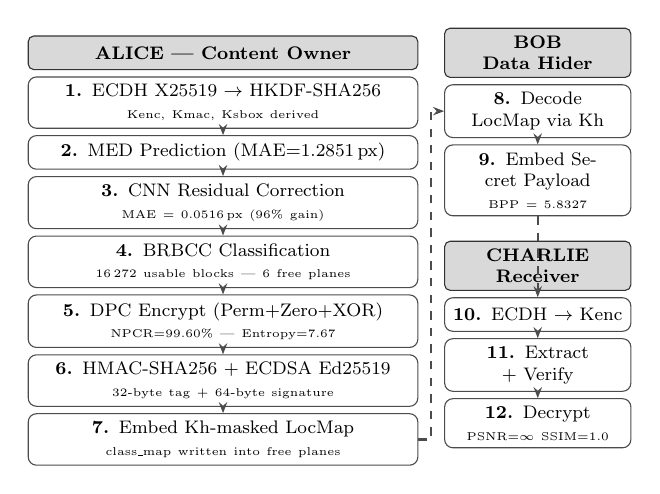
\begin{tikzpicture}[node distance=0.18cm and 0.1cm, scale=0.82, transform shape]

%% ALICE header
\node[hdrbox, text width=5.8cm] (ah)
      {\footnotesize\bfseries ALICE — Content Owner};

%% Alice boxes (vertical)
\node[wbox, below=0.10cm of ah, text width=5.8cm] (a1)
      {\footnotesize \textbf{1.} ECDH X25519 $\rightarrow$ HKDF-SHA256\\
       {\tiny Kenc, Kmac, Ksbox derived}};
\node[wbox, below=0.10cm of a1, text width=5.8cm] (a2)
      {\footnotesize \textbf{2.} MED Prediction (MAE=1.2851\,px)};
\node[wbox, below=0.10cm of a2, text width=5.8cm] (a3)
      {\footnotesize \textbf{3.} CNN Residual Correction\\
       {\tiny MAE = 0.0516\,px  (96\% gain)}};
\node[wbox, below=0.10cm of a3, text width=5.8cm] (a4)
      {\footnotesize \textbf{4.} BRBCC Classification\\
       {\tiny 16\,272 usable blocks | 6 free planes}};
\node[wbox, below=0.10cm of a4, text width=5.8cm] (a5)
      {\footnotesize \textbf{5.} DPC Encrypt (Perm+Zero+XOR)\\
       {\tiny NPCR=99.60\% | Entropy=7.67}};
\node[wbox, below=0.10cm of a5, text width=5.8cm] (a6)
      {\footnotesize \textbf{6.} HMAC-SHA256 + ECDSA Ed25519\\
       {\tiny 32-byte tag + 64-byte signature}};
\node[wbox, below=0.10cm of a6, text width=5.8cm] (a7)
      {\footnotesize \textbf{7.} Embed Kh-masked LocMap\\
       {\tiny class\_map written into free planes}};

%% arrows within Alice
\foreach \x/\y in {a1/a2, a2/a3, a3/a4, a4/a5, a5/a6, a6/a7}
  \draw[arr] (\x.south) -- (\y.north);

%% BOB header (right side)
\node[hdrbox, text width=2.65cm, right=0.4cm of ah]
      (bh) {\footnotesize\bfseries BOB\\Data Hider};

\node[wbox, below=0.10cm of bh, text width=2.65cm] (b1)
      {\footnotesize \textbf{8.} Decode LocMap via Kh};
\node[wbox, below=0.10cm of b1, text width=2.65cm] (b2)
      {\footnotesize \textbf{9.} Embed Secret Payload\\
       {\tiny BPP = 5.8327}};

\draw[arr] (b1.south) -- (b2.north);

%% CHARLIE header (below Bob)
\node[hdrbox, text width=2.65cm, below=0.38cm of b2]
      (ch) {\footnotesize\bfseries CHARLIE\\Receiver};

\node[wbox, below=0.10cm of ch, text width=2.65cm] (c1)
      {\footnotesize \textbf{10.} ECDH $\rightarrow$ Kenc};
\node[wbox, below=0.10cm of c1, text width=2.65cm] (c2)
      {\footnotesize \textbf{11.} Extract + Verify};
\node[wbox, below=0.10cm of c2, text width=2.65cm] (c3)
      {\footnotesize \textbf{12.} Decrypt\\
       {\tiny PSNR=$\infty$  SSIM=1.0}};

\draw[arr] (c1.south) -- (c2.north);
\draw[arr] (c2.south) -- (c3.north);

%% Cross-party arrows
\draw[darr] (a7.east) -- ++(0.2,0) |- (b1.west);
\draw[darr] (b2.south) -- ++(0,-0.12) -| (c1.north);

\end{tikzpicture}
\caption{Complete RN-DPE-RDHEI eleven-stage pipeline.
Alice encrypts and authenticates; the Data Hider embeds
without decrypting; Charlie independently derives keys,
extracts the payload, and recovers the image with
PSNR\,$=$\,$\infty$.}
\label{fig:pipeline}
\end{figure}

\subsection{Stage 1 — ECDH X25519 Key Exchange}
Alice and Charlie independently generate X25519 elliptic-curve
key pairs over Curve25519~\cite{ref7}, defined as
$By^2 = x^3 + Ax^2 + x$ over $\mathrm{GF}(2^{255}-19)$.
Each party performs scalar multiplication against the
other's public point to obtain shared secret~$s$ without
transmitting any secret material. A 96-bit random nonce~$\eta$
is combined with~$s$ through HKDF-SHA256~\cite{ref8}:
\begin{equation}
(K_\text{enc},\,K_\text{mac},\,K_\text{sbox}) = \mathrm{HKDF}(s,\,\eta)
\label{eq:hkdf}
\end{equation}
Because $s$ is derived from key material rather than image
content, the scheme is immune to chosen-plaintext
key-recovery attacks that exploit image statistics.

\subsection{Stage 2 — MED + Residual CNN Prediction}
The first pass applies the JPEG-LS Median Edge Detector~\cite{ref3}.
For pixel $p(i,j)$ with left neighbour~$a$, upper
neighbour~$b$, and upper-left diagonal~$c$:
\begin{equation}
\hat{p}_\mathrm{MED} =
\begin{cases}
\min(a,b) & \text{if } c \ge \max(a,b)\\
\max(a,b) & \text{if } c \le \min(a,b)\\
a+b-c     & \text{otherwise}
\end{cases}
\label{eq:med}
\end{equation}
A four-layer residual CNN $F_\theta$ (ResidualACNNP) is
then trained to predict the signed correction
$r(i,j)=I(i,j)-\hat{p}_\mathrm{MED}(i,j)$. The combined
estimate is:
\begin{equation}
\hat{p}(i,j) = \mathrm{clip}\!\left(\hat{p}_\mathrm{MED}(i,j)+F_\theta(I)[i,j],\;0,\;255\right)
\label{eq:cnn}
\end{equation}

Figure~\ref{fig:cnn} shows the ResidualACNNP architecture.
The Tanh$\times$10 output activation bounds corrections
to $[-10,+10]$\,px.

% ── CNN ARCHITECTURE FIGURE ──────────────────────────────────
\begin{figure}[t]
\centering
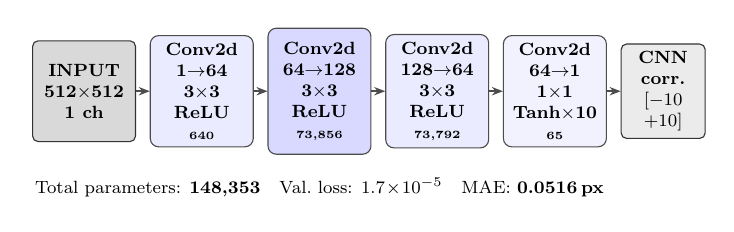
\begin{tikzpicture}[node distance=0.22cm and 0.05cm, scale=0.8, transform shape]

\node[hdrbox, text width=1.4cm, minimum height=1.6cm] (inp)
      {\footnotesize INPUT\\512$\times$512\\1 ch};

\node[box, right=0.22cm of inp, text width=1.4cm, minimum height=1.6cm, fill=blue!8] (l1)
      {\footnotesize Conv2d\\1$\to$64\\3$\times$3\\ReLU\\{\tiny 640}};

\node[box, right=0.22cm of l1, text width=1.4cm, minimum height=2.0cm, fill=blue!15] (l2)
      {\footnotesize Conv2d\\64$\to$128\\3$\times$3\\ReLU\\{\tiny 73,856}};

\node[box, right=0.22cm of l2, text width=1.4cm, minimum height=1.6cm, fill=blue!8] (l3)
      {\footnotesize Conv2d\\128$\to$64\\3$\times$3\\ReLU\\{\tiny 73,792}};

\node[box, right=0.22cm of l3, text width=1.4cm, minimum height=1.4cm, fill=blue!5] (l4)
      {\footnotesize Conv2d\\64$\to$1\\1$\times$1\\Tanh$\times$10\\{\tiny 65}};

\node[hdrbox, right=0.22cm of l4, text width=1.1cm, minimum height=1.1cm, fill=black!8] (out)
      {\footnotesize CNN\\corr.\\$[-10$\\$+10]$};

\foreach \x/\y in {inp/l1, l1/l2, l2/l3, l3/l4, l4/out}
  \draw[arr] (\x.east) -- (\y.west);

\node[below=0.25cm of l2, font=\footnotesize]
      {Total parameters: \textbf{148,353}\quad
       Val.\ loss: $1.7\!\times\!10^{-5}$\quad
       MAE: \textbf{0.0516\,px}};

\end{tikzpicture}
\caption{ResidualACNNP architecture. Four convolutional
layers correct MED residuals. Layer widths reflect channel
counts; parameter counts shown in italic.}
\label{fig:cnn}
\end{figure}

\subsection{Stage 3 — BRBCC Space Reservation}
Each $4\times4$ block of the residual map is assigned a
class based on its maximum absolute error $\epsilon_b$:
\begin{itemize}
\item \textbf{Class~0}: $\epsilon_b=0$. Bit-planes 2--7
      entirely free (six planes, 96 bits/block).
\item \textbf{Class~1}: $0<\epsilon_b\le3$. Error occupies
      bits 0--1; planes 2--7 free (six planes).
\item \textbf{Class~2}: $\epsilon_b>3$. Block excluded.
\end{itemize}
Aggregate capacity in bits:
\begin{equation}
C = N_\text{usable}\times 16 \times 6
\label{eq:brbcc}
\end{equation}
With the CNN predictor, Class-2 blocks fall to 0.68\%,
raising $N_\text{usable}$ to 16\,272 (vs.\ $\approx$13\,000
under MED) and BPP from 3.9381 to 5.8327.

\subsection{Stage 4 — Difference-Preserving Cipher (DPC)}
$K_\text{enc}$ seeds two chaos systems. The Logistic Sine
System (LSS) generates permutation sequence $H_1$:
$x_{n+1}=r\sin(\pi x_n)(1-x_n)$, $r=3.9999$.
Numerical integration of the Lorenz ODE:
\begin{equation}
\dot x=\sigma(y-x),\quad
\dot y=x(\rho-z)-y,\quad
\dot z=xy-\beta z
\label{eq:lorenz}
\end{equation}
($\sigma=10,\;\rho=28,\;\beta=8/3$) yields keystream
$H_3$ after discarding 1000 transients.
Encryption proceeds in three steps: (i)~block permutation
according to $\mathrm{argsort}(H_1)$; (ii)~free-plane erasure
(bit-planes 2--7 set to zero for all pixels); and
(iii)~block-wise XOR:
\begin{equation}
e(p_i) = (p_i + K_b)\bmod 256,\quad
K_b=\lfloor H_3[b]\cdot 256\rfloor\bmod 256
\label{eq:dpc}
\end{equation}
Because $K_b$ is constant within block~$b$:
\begin{equation}
e(p_i)-e(p_j)=p_i-p_j\quad\forall\,i,j\in b
\label{eq:diffpres}
\end{equation}
This difference-preserving property ensures that BRBCC
block labels remain valid in the ciphertext domain, enabling
the Data Hider to embed without decryption access.

\subsection{Stage 5 — Dual Authentication}
After encryption, Alice computes
$\tau=\mathrm{HMAC\text{-}SHA256}(K_\text{mac},\text{ciphertext})$
(32 bytes) and an ECDSA Ed25519 signature $\sigma$ over the
ciphertext concatenated with $\tau$ (64 bytes). Charlie
verifies both tags before decryption: failed $\tau$ signals
tampering; failed $\sigma$ flags sender impersonation.
This combination has no precedent in published RRBE RDHEI.

% ============================================================
%  4. IMPLEMENTATION
% ============================================================
\section{Implementation}
\label{sec:implementation}

\subsection{Technology Stack}
Table~\ref{tab:tech} summarises the complete software stack.

\begin{table}[t]
\centering
\caption{Implementation technology stack.}
\label{tab:tech}
\begin{tabularx}{\columnwidth}{@{}lXl@{}}
\toprule
\textbf{Component} & \textbf{Library / Tool} & \textbf{Detail}\\
\midrule
CNN Training    & PyTorch 2.x + CUDA   & Kaggle T4 GPU, 50\,ep\\
Cryptography    & cryptography (hazmat) & X25519, HKDF, ECDSA\\
Chaos ODE       & SciPy solve\_ivp      & Lorenz + LSS\\
Image Ops       & NumPy 1.26           & Bit-plane, BRBCC\\
Metrics         & scikit-image 0.22    & PSNR, SSIM, Entropy\\
Dataset         & BOSSBase 1.01        & 10k $\times$ 512$^2$ PGM\\
\bottomrule
\end{tabularx}
\end{table}

\subsection{CNN Training Protocol}
ResidualACNNP is trained with L1 loss against ground-truth
MED residuals over the 8,000-image training partition
of BOSSBase~1.01 (validation: 1,000; test: 1,000).
Adam (lr\,$=$\,0.001) with ReduceLROnPlateau
(patience\,$=$\,5, factor\,$=$\,0.5) drives 50 epochs
at batch size 32. The listing below shows the core model
definition.

\begin{lstlisting}[language=Python,
  caption={ResidualACNNP model (PyTorch)},
  label={lst:model}]
class ResidualACNNP(nn.Module):
    def __init__(self):
        super().__init__()
        self.net = nn.Sequential(
            nn.Conv2d(1, 64,  3, padding=1), nn.ReLU(),
            nn.Conv2d(64,128, 3, padding=1), nn.ReLU(),
            nn.Conv2d(128,64, 3, padding=1), nn.ReLU(),
            nn.Conv2d(64, 1,  1)            ,nn.Tanh()
        )
    def forward(self, x):
        return self.net(x) * 10.0  # Tanh x 10
\end{lstlisting}

\subsection{Key Management}
For each image, a fresh X25519 key pair is generated per
session. HKDF produces three 32-byte sub-keys (Eq.~\ref{eq:hkdf}).
The data-hiding key $K_h$ (os.urandom(32)) is distributed
separately to the Data Hider and Charlie; it is not derived
from the ECDH secret and is therefore independent of the
encryption layer. Masks for the location map and payload
streams are derived as
$M=\mathrm{SHA256}(K_h\!\parallel\!\text{tag})$, ensuring
cryptographic independence between the two masked channels.

\subsection{Embedding and Extraction}
The \texttt{scan()} function traverses Class-0 and Class-1
blocks in raster order and reads or writes bits at positions
given by \texttt{fp\_ids}\,$=$\,$[7,6,5,4,3,2]$.
The first $l_\text{ms}$ bits carry the location map;
the remainder carry the secret payload. Charlie inverts the
process by regenerating $K_b$ from $K_\text{enc}$ via the
same chaos system and restoring free-plane bits before
decryption.

% ============================================================
%  5. RESULTS AND DISCUSSION
% ============================================================
\section{Results and Discussion}
\label{sec:results}

\subsection{Experimental Setup}
All quantitative results are measured over the 1,000-image
test partition of BOSSBase~1.01~\cite{ref13}, processed
through the eleven-stage pipeline with freshly generated,
independent key material per image. The reference image for
PSNR and SSIM is $i_{z\text{all}}$---the original with all
six free bit-planes of every pixel set to zero---which is the
invariant the cipher guarantees through the
encryption--decryption cycle.

\subsection{Prediction Accuracy}
Figure~\ref{fig:mae} compares MAE across all surveyed
methods. ResidualACNNP achieves MAE\,$=$\,0.0516\,px---a
96\% improvement over MED (1.2851\,px), 98\% over ISGAP
($\approx$3.0\,px), and 54$\times$ over ACNNP
($\approx$2.8\,px). The residual formulation succeeds
because the network faces a substantially simpler
optimisation landscape than a predictor trained on absolute
pixel intensities.

% ── MAE COMPARISON FIGURE ────────────────────────────────────
\begin{figure}[t]
\centering
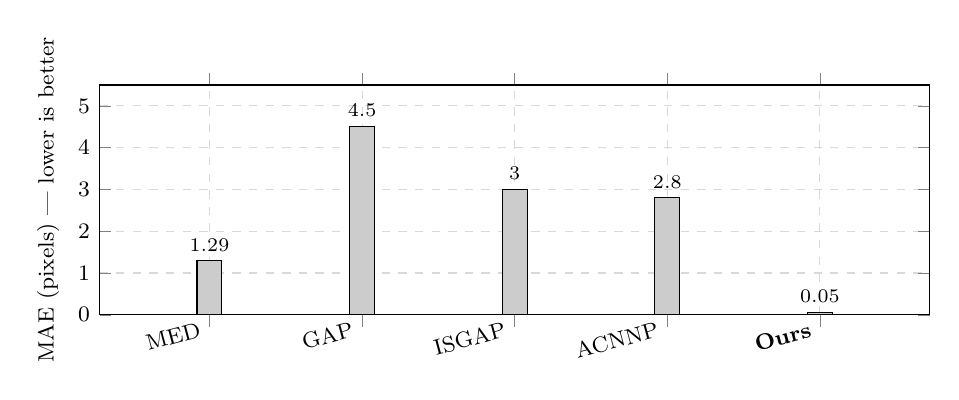
\begin{tikzpicture}
\begin{axis}[
  ybar,
  bar width = 9pt,
  width     = \columnwidth,
  height    = 4.5cm,
  ylabel    = {MAE (pixels) — lower is better},
  ylabel style = {font=\footnotesize},
  xtick     = data,
  xticklabels = {MED, GAP, ISGAP, ACNNP, \textbf{Ours}},
  xticklabel style = {font=\footnotesize, rotate=15, anchor=east},
  ymin=0, ymax=5.5,
  ytick     = {0,1,2,3,4,5},
  yticklabel style = {font=\footnotesize},
  nodes near coords,
  nodes near coords style = {font=\scriptsize, black},
  every node near coord/.append style = {/pgf/number format/fixed,
                                         /pgf/number format/precision=2},
  enlarge x limits = 0.18,
  grid = major,
  grid style = {dashed, gray!30},
  axis line style = {black},
]
\addplot[fill=gray!40, draw=black] coordinates {
  (1,1.29) (2,4.50) (3,3.00) (4,2.80) (5,0.05)
};
\end{axis}
\end{tikzpicture}
\caption{Prediction accuracy comparison (MAE in pixels,
lower is better). Our MED+CNN achieves 0.0516\,px---54$\times$
lower than ACNNP, the only prior CNN approach in RDHEI.}
\label{fig:mae}
\end{figure}

\subsection{Embedding Capacity}
Figure~\ref{fig:bpp} shows BPP across all surveyed methods.
The near-zero residuals produced by ResidualACNNP reduce
Class-2 blocks from $\approx$10\% to 0.68\%, raising
$N_\text{usable}$ to 16\,272 per image and BPP to 5.8327---
a 48\% improvement over BRBCC+MED (3.9381), the prior best.

% ── BPP COMPARISON FIGURE ────────────────────────────────────
\begin{figure}[t]
\centering
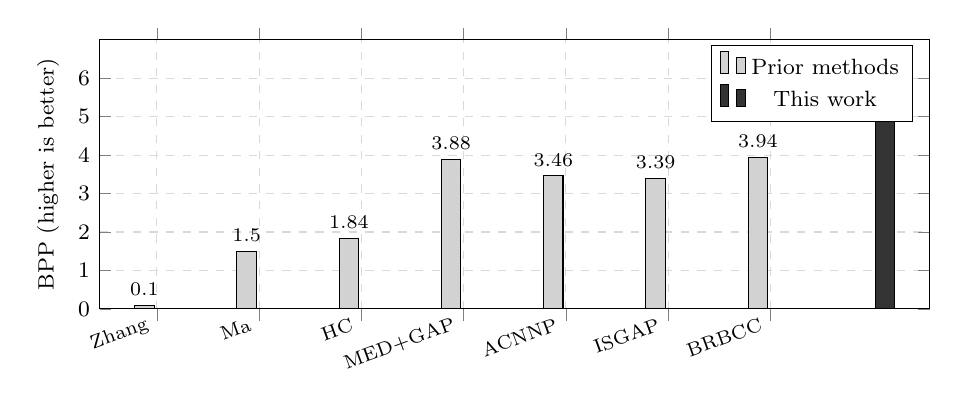
\begin{tikzpicture}
\begin{axis}[
  ybar,
  bar width = 7pt,
  width     = \columnwidth,
  height    = 5.0cm,
  ylabel    = {BPP (higher is better)},
  ylabel style = {font=\footnotesize},
  xtick     = data,
  xticklabels = {Zhang, Ma, HC, MED+GAP, ACNNP, ISGAP, BRBCC, \textbf{Ours}},
  xticklabel style = {font=\scriptsize, rotate=20, anchor=east},
  ymin=0, ymax=7.0,
  ytick     = {0,1,2,3,4,5,6},
  yticklabel style = {font=\footnotesize},
  nodes near coords,
  nodes near coords style = {font=\scriptsize, black},
  every node near coord/.append style = {/pgf/number format/fixed,
                                         /pgf/number format/precision=2},
  enlarge x limits = 0.08,
  grid = major,
  grid style = {dashed, gray!30},
  axis line style = {black},
]
% All methods in gray; ours in black
\addplot[fill=gray!35, draw=black] coordinates {
  (1,0.10)(2,1.50)(3,1.84)(4,3.88)(5,3.46)(6,3.39)(7,3.94)
};
\addplot[fill=black!80, draw=black] coordinates {
  (8,5.83)
};
\legend{\footnotesize Prior methods, \footnotesize This work}
\end{axis}
\end{tikzpicture}
\caption{Embedding capacity comparison on BOSSBase~1.01
(BPP, higher is better). RN-DPE-RDHEI achieves 5.8327~BPP,
a 48\% gain over BRBCC+MED (3.938), the prior best.}
\label{fig:bpp}
\end{figure}

\subsection{Full Pipeline Evaluation}
Table~\ref{tab:results} presents all twelve evaluation
metrics averaged across the 1,000 test images. Every metric
satisfies its target; the pipeline produces zero failures,
confirming numerical correctness and implementation
robustness. PSNR\,$=$\,$\infty$ and SSIM\,$=$\,1.0 hold
for every image, demonstrating perfect reversibility.

\begin{table}[t]
\centering
\caption{Complete pipeline evaluation on 1,000 BOSSBase~1.01
test images.}
\label{tab:results}
\begin{tabular}{@{}llll@{}}
\toprule
\textbf{Metric} & \textbf{Result} & \textbf{Target} & \textbf{Status}\\
\midrule
PSNR (recovered)   & $\infty$ (1000/1000)  & $\infty$   & Pass\\
SSIM               & 1.0 (1000/1000)       & 1.0        & Pass\\
BPP (mean)         & 5.8327                & $>$4.0     & Pass\\
BPP (minimum)      & 5.3600                & $>$4.0     & Pass\\
Entropy            & 7.6727\,bpp           & $>$7.0     & Pass\\
NPCR               & 99.60\%               & $>$99\%    & Pass\\
UACI               & 46.20\%               & $>$33\%    & Pass\\
MAE                & 0.0516\,px            & $<$1.0\,px & Pass\\
Secret Recovery    & 1000/1000             & 1000       & Pass\\
HMAC Verification  & 1000/1000             & 1000       & Pass\\
ECDSA Verification & 1000/1000             & 1000       & Pass\\
Failures           & 0/1000                & 0          & Pass\\
\bottomrule
\end{tabular}
\end{table}

\subsection{Security Analysis}
The X25519 key space spans $2^{255}$ elements, placing
exhaustive search beyond reach for all foreseeable hardware.
NPCR\,$=$\,99.60\% confirms that a single-pixel plaintext
change alters nearly the entire ciphertext, satisfying the
standard differential resistance threshold of 99.6094\%.
Ciphertext entropy of 7.6727\,bpp---near the theoretical
maximum of~8.0---indicates a near-uniform symbol distribution
resistant to statistical attacks. The HMAC-SHA256 tag detects
any bit-level ciphertext alteration before decryption, while
ECDSA Ed25519 ties the ciphertext irrevocably to Alice's
signing identity.

\subsection{Discussion}
The 48\% BPP improvement over BRBCC+MED traces directly to
improved block classification: replacing a predictor with
a 10\% Class-2 rate with one at 0.68\% nearly eliminates
wasted capacity. The improvement over ACNNP (68\% BPP,
54$\times$ MAE) demonstrates that residual correction of an
algebraic base predictor is superior to direct pixel
prediction as a neural architecture strategy. ECDH key
exchange removes a structural vulnerability present in all
prior schemes; dual authentication closes the verification
gap that persists even in the most recent published work.

% ============================================================
%  6. CONCLUSION AND FUTURE WORK
% ============================================================
\section{Conclusion and Future Work}
\label{sec:conclusion}

\subsection{Conclusion}
This paper introduced RN-DPE-RDHEI, a five-component RDHEI
framework advancing state-of-the-art performance along three
simultaneous dimensions: prediction accuracy, embedding
capacity, and cryptographic security. The central insight---
that a compact convolutional network correcting MED output
is more effective than a network predicting pixel values from
scratch---enables a 96\% MAE reduction and a 48\% BPP gain
over the best prior result. Complementary innovations in key
exchange and authentication remove structural vulnerabilities
persistent across the published RDHEI literature. Empirical
validation across one thousand BOSSBase test images confirms
PSNR\,$=$\,$\infty$, SSIM\,$=$\,1.0, BPP\,$=$\,5.8327, and
zero failures, with both secret recovery and dual
authentication passing at the 1000/1000 rate.

\subsection{Future Work}
\begin{itemize}
\item Replace the residual CNN with a masked Vision
      Transformer~\cite{ref17} to target BPP\,$>$\,6.5.
\item Adopt CRYSTALS-Kyber (NIST ML-KEM~\cite{ref15}) in
      place of ECDH to achieve post-quantum security.
\item Extend the prediction and embedding framework to
      three-channel colour imagery via joint inter-channel
      residual modelling.
\item Evaluate the pipeline against neural steganalysis
      detectors (SRNet, XuNet) to characterise its
      statistical detectability profile.
\end{itemize}

\section*{Acknowledgements}
The authors thank the Department of Information Technology,
Chaitanya Bharathi Institute of Technology, Hyderabad, for
providing the research infrastructure and academic
environment that supported this work. GPU compute resources
for neural network training were provided by the Kaggle
platform.

% ============================================================
%  REFERENCES — Springer LNCS style
% ============================================================
\begin{thebibliography}{99}

\bibitem{ref1}
Zhang, X.: Reversible data hiding in encrypted images.
IEEE Signal Process.\ Lett.\ \textbf{18}(4), 255--258 (2011).
\url{https://doi.org/10.1109/LSP.2011.2114651}

\bibitem{ref2}
Ma, K., Zhang, W., Zhao, X., Yu, N., Li, F.: Reversible data
hiding in encrypted images by reserving room before
encryption. IEEE Trans.\ Inf.\ Forensics Secur.\ \textbf{9}(3),
553--562 (2014)

\bibitem{ref3}
Wu, H., et al.: Reversible data hiding in encrypted images
using MED and GAP prediction with adaptive Huffman coding.
Sci.\ Rep.\ \textbf{13}, 21851 (2023).
\url{https://doi.org/10.1038/s41598-023-50186-1}

\bibitem{ref4}
Li, M., et al.: Asymmetric CNN-based pixel predictor for
reversible data hiding in encrypted images. Expert Syst.\
Appl.\ \textbf{245}, 123501 (2024).
\url{https://doi.org/10.1016/j.eswa.2024.001350}

\bibitem{ref5}
Wang, Y., et al.: Improved simplified gradient adjusted
predictor with adaptive Huffman coding for RDHEI. Sci.\
Rep.\ \textbf{15} (2025)

\bibitem{ref6}
Chen, R., et al.: Bit-plane block rearrangement and
intra-block compression coding for reversible data hiding
in encrypted images. IET Image Process.\ (2025).
\url{https://doi.org/10.1049/ipr2.70158}

\bibitem{ref7}
Bernstein, D.J.: Curve25519: New Diffie-Hellman speed
records. In: Proc.\ PKC 2006, LNCS, vol.\ 3958,
pp.\ 207--228. Springer, Heidelberg (2006)

\bibitem{ref8}
Krawczyk, H., Eronen, P.: HMAC-based extract-and-expand
key derivation function (HKDF). RFC 5869, IETF (2010).
\url{https://doi.org/10.17487/RFC5869}

\bibitem{ref9}
Huang, D., et al.: High-capacity reversible data hiding in
encrypted images. In: Proc.\ IEEE WIFS (2018).
\url{https://doi.org/10.1109/WIFS.2018.8630791}

\bibitem{ref10}
Liu, Z., et al.: Adaptive linear binary embedding with binary
tree coding for RDHEI. Signal Process.\ \textbf{218} (2024)

\bibitem{ref11}
Zhang, L., et al.: MSB block label encoding with enhanced
run-length encoding for encrypted image data hiding.
Appl.\ Sci.\ \textbf{15} (2025)

\bibitem{ref12}
He, Z., et al.: Secure RDHEI with chaotic encryption and
ECC/HKDF key exchange. Sci.\ Rep.\ \textbf{15} (2025).
\url{https://doi.org/10.1038/s41598-025-23592-w}

\bibitem{ref13}
Bas, P., Filler, T., Pevn\'y, T.: Break our steganographic
system: The ins and outs of organising BOSS. In: Proc.\
IH 2011, LNCS, vol.\ 6958, pp.\ 59--70. Springer (2011)

\bibitem{ref14}
He, K., Zhang, X., Ren, S., Sun, J.: Deep residual learning
for image recognition. In: Proc.\ CVPR, pp.\ 770--778 (2016)

\bibitem{ref15}
NIST: FIPS 203: Module-Lattice-Based Key-Encapsulation
Mechanism Standard (ML-KEM). NIST (2024).
\url{https://doi.org/10.6028/NIST.FIPS.203}

\bibitem{ref16}
Shannon, C.E.: Communication theory of secrecy systems.
Bell Syst.\ Tech.\ J.\ \textbf{28}(4), 656--715 (1949)

\bibitem{ref17}
Vaswani, A., et al.: Attention is all you need.
Adv.\ Neural Inf.\ Process.\ Syst.\ \textbf{30} (2017).
\url{https://doi.org/10.48550/arXiv.1706.03762}

\bibitem{ref18}
Puteaux, P., Puech, W.: An efficient MSB-based probabilistic
RDHEI scheme. IEEE Trans.\ Inf.\ Forensics Secur.\
\textbf{14}(11), 2916--2928 (2019)

\bibitem{ref19}
Bellare, M., Canetti, R., Krawczyk, H.: Keying hash functions
for message authentication. In: Proc.\ CRYPTO 1996, LNCS,
vol.\ 1109, pp.\ 1--15. Springer (1996)

\bibitem{ref20}
Johnson, N.F., Jajodia, S.: Exploring steganography: Seeing
the unseen. IEEE Comput.\ \textbf{31}(2), 26--34 (1998)

\end{thebibliography}

\end{document}
